\chapter{Language Overview}
\label{chp:concepts}

% \section{Overview of SBGN \PDs}
\label{sec:PD-overview}

 To briefly describe what SBGN \PDl is about, let's give a brief overview of some of the relevant concepts with the help of an example shown in \fig{eg1}. It is a simple map for part of a mitogen-activated protein kinase (MAPK) cascade.  The larger nodes in the figure (some of which are in the shape of rounded rectangles and others in the shape of circles) represent biological materials---things like macromolecules and simple chemicals (NB: the nodes representing physical entities (or proxies to physical entities) will always be colored in yellow in this document. Color is not part of the SBGN specification though).
% % [!] yellow is not just for EPNs, it is also occasionally used for glyphs such as stoichiometry labels, modulation arrowheads, compartments, logical operators and units of information (when introducing these glyphs). Is the explanation on colors clear enough? (e.g. also the fact they are not part of the specs, but still allowed?). Should this explanation be expanded a bit in a short paragraph of its own? Or at least a different sentence? I did find the parenthesis a bit distracting the first time I read this paragraph.
 The biological materials are altered via processes (colored in green in this document), which are indicated in \PDl by lines with arrows and other decorations.  In this particular map, all of the processes happen to be the same: processes catalyzed by biochemical entities.
 The directions of the arrows indicate the direction of the processes; for example, unphosphorylated RAF kinase proceeds to phosphorylated RAF kinase via a process catalyzed by RAS. Although ATP and ADP are shown as incidental to the phosphorylations on this particular graph, they are involved in the same process as the proteins getting
 phosphorylated. The small circles on the nodes for RAF and other entity pools represent state variables (in this case, phosphorylation sites).

% Redo the figure with colors
\begin{figure}[htb]
  \centering
  \vspace*{-0.75em}
  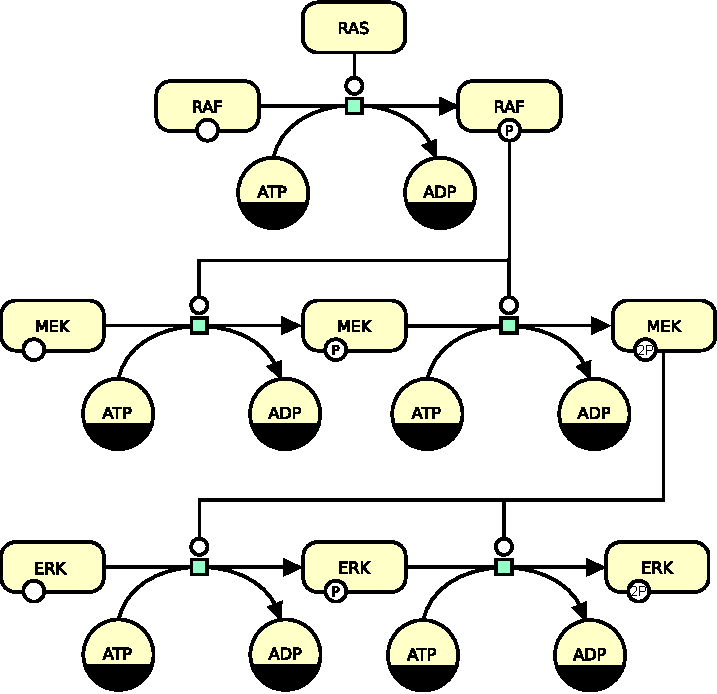
\includegraphics[scale=0.8]{images/MAPK-only}
  \caption{This example of a \PD uses two kinds of entity pool nodes: one for pools of different macromolecules (\sect{techref:macromolecule}) and another for pools of simple chemicals (\sect{techref:simpleChemical}). Most macromolecule nodes in this map are adorned with state variables (\sect{techref:stateVariable}) representing phosphorylation states. This map uses one type of process node, the process node (\sect{techref:process}), and three kind of connecting arc, consumption (\sect{techref:consumption}), production (\sect{techref:production}) and catalysis (\sect{techref:catalysis}).  Finally, some entity pool nodes have dark bands along their bottoms; these are clone markers (\sect{techref:cloneMarker}) indicating that the same pool nodes appear multiple times in the map.}
  \label{fig:eg1}
\end{figure}

The essence of the \PDs is \emph{change}: it shows how different entities in the system process from one form to another.  The entities themselves can be many different things.  In the example of \fig{eg1}, they are either pools of macromolecules or pools of simple chemicals, but as will become clear later in this chapter, they can be other conceptual and material constructs as well.  Note also that we speak of \emph{entity pools} rather than individuals; this is because in biochemical network models, one does not focus on single molecules, but rather collections of molecules of the same kind.  The molecules in a given pool are considered indistinguishable from each other.  The way in which one type of entity is transformed into another is conveyed by a \emph{process node} and arcs between entity pool nodes and process nodes indicate an influence by the entities on the processes.  In the case of \fig{eg1}, those arcs describe consumption (\sect{techref:consumption}), production (\sect{techref:production}) and catalysis
(\sect{techref:catalysis}), but others are possible.  Finally, nodes in \PDs are usually not repeated; if they do need to be repeated, they are marked with \emph{clone markers}---specific modifications to the appearance of the node (\sect{techref:cloneMarker}). The details of this and other aspects of \PD notation are explained in the rest of this chapter.

A reference card depicting all the symbols of \SBGNPDLone is present at the end of this document.

Lets look at a few additional examples which show typical biological processes and their SBGN \PD representation. In \fig{eg2} a reversible reaction with two substrates and one product is shown. The enzyme E catalyzes an irreversible (metabolic) process which consumes two substrates (S1 and S2) and produces one product (P1). The enzyme is a protein, therefore represented as a \emph{macromolecule}. Substrates and product of the biochemical reaction are represented by \emph{simple chemicals}. The consumption of S1 and S2 is represented by the \emph{consumption arcs}. The \emph{production arc} represents the synthesis of P1. 

In \fig{eg3} the formation of a complex is shown. Two \emph{macromolecule} entities X and Y form the \emph{complex} X\underline{ }Y. Complex formation is represented using the \emph{association} process node with ingoing \emph{consumption} and outgoing \emph{production} arcs. The \emph{complex} glyph surrounds subunits X and Y.

\begin{figure}[htb]
  \centering
  \vspace*{-0.75em}
  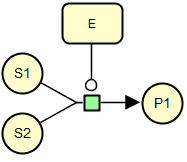
\includegraphics[scale=0.5]{images/Fig12}
  \caption{This example of a \PD shows an irreversible catalysis with 2 substrates and 1 products.}
  \label{fig:eg2}
\end{figure}

\begin{figure}[htb]
  \centering
  \vspace*{-0.75em}
  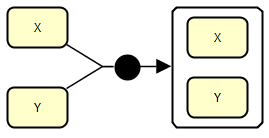
\includegraphics[scale=0.5]{images/Fig13}
  \caption{This example of a \PD shows an irreversible catalysis with 2 substrates and 1 products.}
  \label{fig:eg3}
\end{figure}

In \fig{eg4} the regulation of a target gene by a transcription factor without knowledge about the promoter binding is shown. A transcription factor (TF) protein together with a target gene promoter X triggers the\emph{process} of transcription. Direct binding of the TF to the target gene promoter has not been experimentally verified, therefore the \emph{logical operator} AND is used to describe the yet unspecified interaction between TF and target gene. The TF protein is a \emph{macromolecule} of the \emph{material type} 'protein' (mt:prot) whereas the gene promoter is given as a \emph{nucleic acid feature} with the \emph{conceptual type} 'gene' (ct:gene). The connecting arc \emph{necessary stimulation} is applied to indicate that the stimulation by both regulator and target is necessary for the transcription process to take place. The target gene messenger as a product of the transcription process is represented by a \emph{nucleic acid feature} with the \emph{conceptual type} 'mRNA' (ct:mRNA). The \emph{unspecified source} symbol is used to represent the large number of substrates of a transcription process (i.e. trinucleotides).

A last example is show in \fig{eg5}, which shows passive transport or diffusion of a molecule. The \emph{macromolecule} X in the cytosol serves as the substrate of a process leading to the production of the \emph{macromolecule} X in the nucleus. This process describes the passive transport of X from one \emph{compartment} to the other. The two macromolecules X do not carry the clone marker because the containing compartment is part of their identity.

More examples can be found in a list of so called SBGN bricks~\cite{Junker:2012}, which are building blocks representing basic biological patterns. These bricks can be used for assembly into different kinds of biological networks such as metabolic and regulatory networks.

\begin{figure}[htb]
  \centering
  \vspace*{-0.75em}
  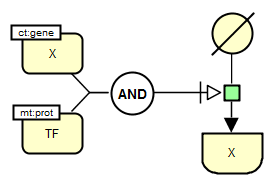
\includegraphics[scale=0.5]{images/Fig14}
  \caption{This example of a \PD shows a regulation of a target gene by a transcription factor without knowledge about the promoter binding.}
  \label{fig:eg4}
\end{figure}


\begin{figure}[htb]
  \centering
  \vspace*{-0.75em}
  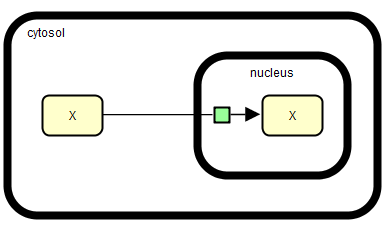
\includegraphics[scale=0.5]{images/Fig15}
  \caption{This example of a \PD shows a passive transport of a molecule.}
  \label{fig:eg5}
\end{figure}

%\section{Some more concept text}

% \SBGNPDLone is a visual language. Like any language like English it has a vocabulary, which in the case of SBGN is represented by the symbols that we call glyphs. Again like English our language has grammar, which are the underlying rules and concepts of the language that define its meaning. This specification aims to provide a detailed description of both the vocabulary and grammar rules of the language as a reference. However, to understand this it is essential to grasp what an \PDm describes.

% The first thing to understand is the SBGN-PD does not describe biochemical reactions or gene expression --- at least not directly. Instead this language describes collections --- pools --- of entities that are manipulated by processes which can convert them from one type of entity to another. An entity pool that is the input to a process is said to consumed and that which is an output is produced. There is a third class of entity pool associated with a process: namely those that affect --- modulate --- the rate at which a process converts entity from one set of pools to another. The amount of entity in a modulating pools is not changed by the process. These very briefly are the key concepts of PD and are illustrated in figure \ref{fig:keyconcepts}.

% \begin{figure}[htb]
% \begin{center}
% \scalebox{0.5}{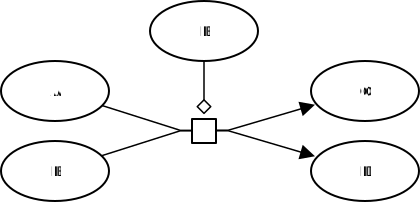
\includegraphics{images/keyconcepts}}
% \caption{A process consuming the entity pools A and B and producing the entity pools C and D. The entity pool E modulates the process. The process is represented as a square. Each (unspecified) entity pool is represented as an ellipsis identified by a label. The relationships between the process and each entity pool involved are represented by connecting lines called arcs. Depending on the type of relationship (consumption, production, modulation), these arcs are decorated with different symbols (respectively nothing, arrowhead, and diamond).}\label{fig:keyconcepts}
% \end{center}
% \end{figure}

% So how do this enable us to describe biological processes? Very simply. Figure \ref{fig:biochem} illustrates a biochemical reaction and shows how the essential components of that reaction, substrate, product and enzyme catalyst are all conveniently described by the representation. Likewise in figure \ref{fig:genereg} we can see again the concept of entity pools and process flow can be applied to gene regulation. This approach gives us a lot of flexibility and enables one to summarise biological processes that may incorporate many biochemical reactions (figure \ref{fig:summarisingproc}).


%%% Diff EPN & Process types here.

In the above examples of biological processes a number of different glyphs where used to illustrate different biological entities: the macromolecule, the simple chemical and the gene.


%%% Compartments.


%%% Clone markers and identity

%%% Logic gates

%%% Maps & Submaps


%%%Overview of the UML/Class specification. 

% \subsection{Graph, diagram or map?}

% A graph is a very technical term that belongs to mathematics and is uncommon in biology. Diagram is a concept that encompasses more than just graph. Examples are Venn diagrams for instance. Therefore, we recommend using the term map for SBGN representations. Those representations effectively permit users to travel and orient themselves in a biological system. Map is also the term most frequently used by the different communities, whether in metabolism, signaling or genomics.


